\externaldocument[I-]{MaxHughesThesis}

In order to get a measurement of the Fierz term, the spectrum shape needed to get fit.
The effect of bremstrahlung and the effieciency of the detectors needed to be accounted for.
The way this was done was with a a simulation.

\section{GEANT4 Monte Carlo}
The corrected beta decay spectrum was fed as input to a Monte Carlo.
The program used to model the detectors was GEANT4.
In order to use the program, parameters must be introduced.

\subsection{Detector Simulation}
The geometry of the detector set-up was programmed into the simulation.
The implant detector was modeled as a square prism of CsI.
The rectangular prism was 9.76 cm deep with a 5 cm square base.
The front edge implant detector was put at the center of the simulation.
The aluminum sheath and MgO layer was not simulated for the implant detector.

The four large gamma detectors also square prisms.
The active volume was 79.5 mm square and 76.2 mm deep.
It was also made of CsI.
Around this detector, a 1.5 mm laywer of MgO was added.
On top of this, the can of aluminum, 1 mm thick, was added into the simulation.

The four large gamma detectors were arranged into a square around the implant detector.
Each square base of the gamma detectors was centered one inch upstream from the face of the implant detector.
This modeled how the implant detector was recessed in the experiment. 

\subsection{Source Definition}
The next step was to define a region inside the implant detector.
This region was where the gamma and beta particles orignated from.
The depth of the region was calculated using LISE++, a ion optics code.
The verticle and horizontal size of the region was calulated by using the PPAC measurement and an ion optics simulation.
This size was 0.4 mm deep, 3.5 mm wide, and 3.6 mm tall.
The source was implanted 1.156 cm into the detector.

Once these parameters were known, GEANT4 was told to generate two particles.
First, the corrected beta energy spectrum was sampled and an electron of that energy was generated inside the implant region.
The beta energy spectrum was generated using all the corrections described in chapter \ref{ch:theory}. 
The location of the electron was recovered, and a photon with an energy of  1.6 MeV was generated as well.
The initital direction of the two particles was as isometric.
These particles where then propagated through the detector setup..
GEANT4 uses a physics list that has all the interactions a particle could take.
The physics list used was standard option 4.
This list is better at low energy electron physics. 

\subsection{Primary Particle Definitions}
There were three primary particles generated.
Two were photons and one was an electron.
All three particles had an isotropic angular distribution.
The origin points of all the primary particles was the same.

One photon was the 1.6336 MeV photon from the $^{20}$F decay.
The energy of this photon was not changed.

The electron was generated according to phase space spectrum (equation \ref{eq:phase_space}) times all the corrections.
For the radiative correction, the electron was generated with the formala that assumes all real photon energy is absorbed (equation \ref{eq:fayansrad}).
However, this is not exactly true. 
In this case, due to the geometry, photons are absorbed totaly if they are below 100 keV in energy.
In order to properly see the effect of the real photon emmission, the second primary particle is used.

After the electron energy is generated, a formula describing the energy spectrum of the inner bremsstrahlung photons is generated. 
This spectrum is written out in equation \ref{eq:KUB}. % Add KUB again here? Probably.
Further discussion of this formula is found in the theory chapter.
A cutoff of 50 keV is imposed to the formula, as it has a singularity at zero photon energy.
Then, the formula is numerical integrated from 50 keV to the electron energy.
This is the total probablity that an electron emits a KUB photon.
This number is compared to a random number from 0 to 1.
If the random number is below the integral, the inner bremsstrahlung energy spectrum is sampled.
The algorithm used for this sampling is the van Neumann method \cite{neu51}.
The sampled energy is given to the third primary particle.
The energy of the electron is reduced accordingly.

After all three particles have their energies defined, they are propogated through the detector set up.

\subsection{Simulation Results Processing}
The particles were tracked and the energy deposited in each detector summed up.
The energy deposited in the implant detector was further seperated into two parts:
Energy from the  electron and the inner bremstrahlung photon.
Energy from the 1.6336 MeV photon
After the energies of the particles reached a certain threshold, the simulation of one decay was finished.
All the energies deposited into each of the detectors was summed up and saved as an event in a ROOT tree.
Then, the process was repeated.
A new location inside the region was generated and another decay generated.

In order to get to get the necessary statistics, 2 * 10$^{9}$ events had to be generated. 
After the events were done, the simulation data was processed further. 
Much like the experimental data, the simulated data had to be filtered.
The energy absorbed in the implant detector was filtered by the energy absorbed in the outer four gamma detecters in the simulation.

The filtered data was seperated into two parts:
Absorbed energy in the implant detector only orginating from the electron.
Absorbed energy in the implant detector with some contribution from the gamma ray.
These energies were built into two different histograms.
These two histograms had the detector resolution applied to it. 

The convolution function was

\begin{equation}
	\sigma = A\sqrt{E}
	\label{eq:convo}
\end{equation}

where $\sigma$ was the energy resolution, $E$ the energy, and $A$ a constant found through a calibration.

\subsubsection{Pile-up Modelling}
After the convolution, the simulation data was sent through a simulation to model pile-up.
The model used for the CsI(Na) signals was a linear rise and then an exponential decay.
The linear part went from 0 to 1 over 100 ns. 
The exponential piece started at 100 ns at 1 and decayed with a $\tau$ of 760 ns.
This analytic equation was scaled up or down to whatever energy was sampled.
It was then fed into a model of trapezoidal filter of PIXIE. 
The math was the same as described in the chapter on data aquisition.


This model was tuned on calibration data. 
A run was taken of $^{137}$Cs at 25000 counts per second.
A 2000 counts per second $^{137}$Cs run was used as a background and subracted off.
Then, samples of the background-subtracted spectrum were taken up to the end of the 661 keV peak.
Monte Carlo methods were used to model the time difference between two samples.
If the two samples fell within the pile-up window, then the piled-up signal models were fed into the trapezoidal filter.
The calculated pile-up energy was saved to a histogram.
If the two samples did not fall with in the pile-up window, then they were not fed into the filter model and just filled into the histogram.
The paremeters were adjusted until the generated pile-up matched the measured pile-up in the spectrum.
The results of the tuning is seen in figure \ref{fig:pileuptune}

\begin{figure}[!htb]
	\centerline{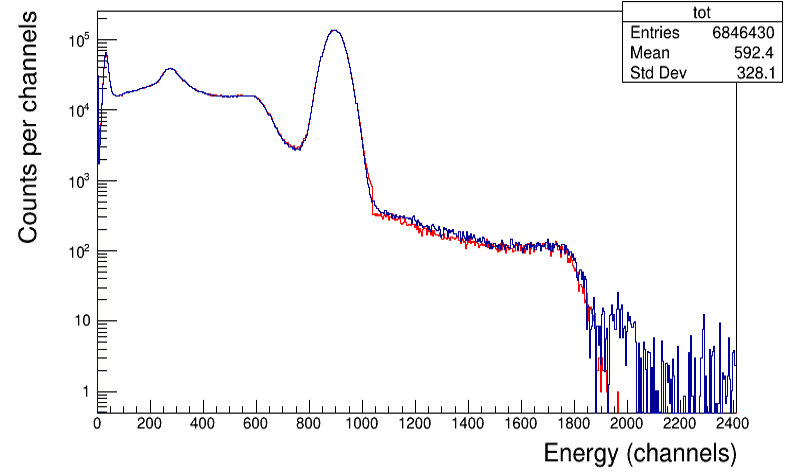
\includegraphics[width=0.78\textwidth]{PileUpTuningThesis.png}}
	\caption{The tuning of the pile-up.
		 The input spectrum is in blue.
		 It was sampled up to 1000 channels.
		 The generated spectrum is in red.}
	\label{fig:pileuptune}
\end{figure}

\section{Calibration}
In order to properly fit the energy spectrum, a calibration of the CsI(Na) detector had to be done.
Several different energy lines were used to find the calibration and the energy resolution function.
The lines were the 1.173228 MeV and 1.332.492 MeV gammas from a $^{60}$Co source, the 0.661657 MeV gamma ray from a$^{137}$Cs source, and the 0.511 MeV and 1.274527 MeV gamma rays from a $^{22}$Na source.
These gamma rays were fitting with a gaussian and a background.
The background varried from a linear background, a quadratic background, and an error function background.
For the $^{60}$Co, both peaks were fit at once.
These different background gave slightly different results for the centroids and the widths of the gaussians.
The different widths and centroids were taken as a systematic error.
From the centroids, the calibration for each detector was calculated and shown in equation \ref{eq:cal}

\begin{equation}
	C = G * E + b
	\label{eq:cal}
\end{equation}

where $C$ is the location of the peak in ADC channels, $G$ the gain in channels/keV, and b the offset in channels.
The widths of the peaks were calibrated with the gain and plotted vs energy.
Then, equation \ref{eq:convo} was fit to the results in order to determine $A$.

\section{Fitting Procedure}
The simulation described above were only part of what was needed.
Other simulations included in the fit had the phase space times corrections times or divided an additional factor of the total energy of the electron.
The simulations were all convoluted and filtered as described above.

\subsection{Data Processing}
The data was processes from the TTrees described in the previous section.
The energy spectrum of the implant detector was put in coincidence with the 4 gamma detectors.
The energy cuts of the gamma detectors were the same as in the life-time measurement.
There was a time difference condition as well.
For this measurement, the time difference between a beta event and a gamma event had to be between -300 and 24 ns.
Then, a 2-D histogram was built, with energy on one axis and time since last beam on on there other.
Since afterglow causes an effect that looks like a gain shift, different time cuts of equal statistics were taken from this 2-D histogram. 
These time cuts were then fit. 
The gain was left as a free parameter to counteract this afterglow effect.

\subsection{Fit Function}
The fit function used was as follows.
First, the x axis of the data was read.
This number was in ADC units, so equation \ref{eq:cal} was used to turn this number into energy in keV.
For the fitting, the gain $G$ was left as a free parameter, but the offset $b$ was set from the calibration.

\begin{equation}
	A * (f(E)_{nosum} * S(E,b_{wm}$) + f(E)_{summing}) + B*p(E)
	\label{eq:betafit}
\end{equation}

where $A$ is the normalization, $B$ the level of pile-up, $E$ the energy, $b_{wm}$ the weak magnetism, $S(E,b_{wm})$ the shape factor, $f(E)_{nosum}$ the output of the GEANT4 simulation without any energy summing between the gamma and beta, and $f(E)_{summing}$ the output of the GEANT4 simulation with energy summing.
The free parameters here are $A$, $B$, and $b_{wm}$.

\subsection{Fit details}
The fit was done run by run.
First a prefit for each section was done to calibrate the energy.
Then, two endpoints in keV were used for the fit.
The fitting function with a fixed offset was fit using a maximum likelyhood method.
The resulting $b_{wm}$ was recorded. 
